\newpage

\section{Разработка архитектурно-структурных решений}

Выполнение кода предметно-ориентированного языка осуществляется за счет интерпретатора,
который должен быть спроектирован в виде модуля, подключаемого к серверной части конструктора Telegram ботов.

Обобщенная модульная структура серверной части конструктора представлена на рисунке~\ref{f:modules_server_struct}.

\begin{figure}[ht]
	\centering
	\vspace{\toppaddingoffigure}
	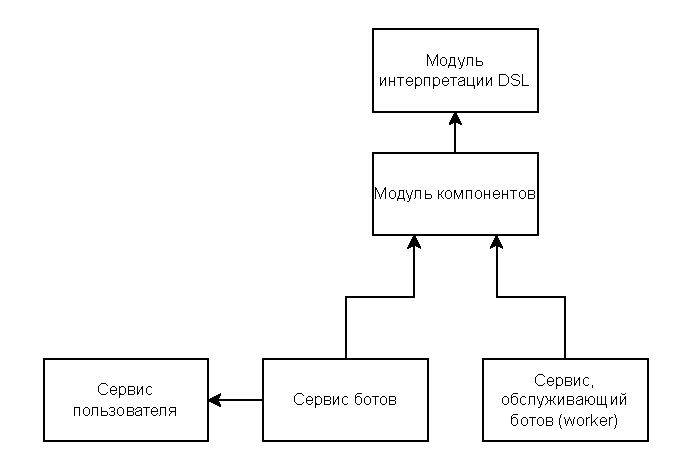
\includegraphics[width=0.7\textwidth]{modules_server_struct.pdf}
	\caption{Модульная структура серверной части конструктора}
	\label{f:modules_server_struct}
\end{figure}

Сервис ботов отвечает за управление состоянием бота и редактирование его компонентной структуры.
Сервис ботов зависит от сервиса пользователей, который предоставляет первому методы для авторизации пользователя.
Также сервис ботов зависит от модуля компонентов, который описывает структуры компонентов и реализует их логику выполнения.

Обслуживающий сервис отвечает за логику работы бота. 
Он выполняет обработку запроса к боту от пользователя Telegram.
В соответствии с разработанной компонентной структурой бота, обслуживающий сервис вызывает методы модуля компонентов для запуска их логики выполнения.

Одним из компонентов является компонент выполнения кода на предметно-ориентированном языке.
Отсюда, модуль компонентов зависит от модуля интерпретации предметно-ориентированного языка.
При запуске компонента выполнения DSL кода, выполняется вызов функции выполнения кода из модуля интерпретации.

Таким образом, в данном проекте для возможности интеграции с серверной частью конструктора Telegram ботов необходимо реализовать программный интерфейс,
который бы предоставлял возможность передачи кода и значений внешних переменных, интерпретатору предметно-ориентированного языка.

Для решения поставленной задачи, в первую очередь, необходимо в соответствии с указанными требованиями
разработать грамматику предметно-ориентированного языка и спроектировать обобщенную структуру программы интерпретатора.


\subsection{Разработка грамматики языка}

Описание языка программирования основывается на теории формальных языков.
В данном разделе проводится разработка формальной грамматики языка.


\subsubsection{Способы задания языков}

Для задания языка можно воспользоваться следующими методами:

\begin{enumerate}
    \item перечислить все цепочки языка;
    \item указать способ порождения цепочек;
    \item определить метод распознавания допустимых цепочек.
\end{enumerate}

Перечисление всех цепочек языка возможно в исключительных случаях, например,
когда для управления некоторой системой достаточно двух-трех команд.

Механизм порождения цепочек предполагает использование формальной порождающей грамматики.

Формальная порождающая грамматикиа -- это математиечская система, описывающая правила построения цепочек некоторого (формального) языка.

Распознавание допустимых цепочек осуществляется с помощью некоторого логического устройства -- распознавателя.
На вход распознавателя подается цепочка, а на выходе образуется логическое значение <<истина>> в случае принадлежности цепочки языку
и <<ложь>>, если цепочка языку не принадлежит.
Распознаватели строятся на основе теорий конечных автоматов и автоматов с магазинной памятью.

Методы порождения и распознавания тесно связаны.
Механизм порождения обычно используется при описании языка, а распозанватель при его реализации, т.е. в трансляторе.

Описать синтаксис языков программирования можно несколькими способами, например, такими как формы Бэкуса-Наура, диаграммы Вирта и другими.
Это методы задают правила вывода, определяющие возможные конструкции цепочек языка.
В данном проекте для описания грамматики языка используется расширенная форма Бэкуса-Наура (РБНФ).



\subsubsection{Применение расширенной формы Бэкуса-Наура для описания формальной грамматики языка}

Расширенная форма Бэкуса-Наура – формальная система определения синтаксиса,
в которой одни синтаксические категории последовательно определяются через другие.
Используется для описания контекстно-свободных грамматик.

Формальная грамматика задаётся четвёркой вида:

\(G = (V_T, V_N, P, S)\),

где \(V_T\) -- множество терминальных символов грамматики – конечные
элементы языка, не разбирающиеся на более мелкие составляющие в рамках
синтаксического анализа, например ключевые слова, цифры, буквы
латинского алфавита.

\(V_N\) -- конечное множество нетерминальных символов – элементов грамматики, имеющих собственные имена и структуру.
Каждый нетерминальный символ состоит из одного или более терминальных и/или нетерминальных символов.

\(P\) -- множество правил вывода грамматики.

\(S\) -- начальный символ грамматики, \(S \in V_N\).

РБНФ является одним из видов формальных грамматик.
РБНФ состоит из множества правил вывода, каждое из которых определяет синтаксис некоторой конструкции языка.

Некоторые основные конструкции РБНФ:

\begin{itemize}
    \item A, B -- конкатенация элементов;
    \item A | B -- выбор (A или B);
    \item {[A]} -- элемент в квадратных скобках может отсутствовать (аналог - <<?>>);
    \item \{A\} -- повторение элемента 0 или более раз (аналог - <<*>>);
    \item (A B) -- группировка элементов;
    \item (* … *) – комментарий;
    \item <<;>> – отмечает окончание правила (аналог - <<.>>).
\end{itemize}

Кроме того, в качестве синтаксического сахара могут использоваться следующие символы:

\begin{itemize}
    \item <<*>> - предыдущий элемент может встречаться 0 или более раз;
    \item <<?>> - предыдущий элемент является необязательным (присутствует 0 или 1 раз);
    \item <<+>> - предыдущий элемент встречается 1 или более раз.
\end{itemize}

В соответствии с данными правилами описание синтаксиса предметно-ориентированного языка будет выглядеть следующим образом:
